\documentclass{article}

\usepackage[T1]{fontenc}
\usepackage{microtype}
\usepackage{graphicx}
\usepackage{booktabs}
\usepackage{array}
\usepackage{amsmath}
\usepackage{amssymb}
\usepackage{hyperref}
\setlength{\emergencystretch}{2em}

\newcommand{\theHalgorithm}{\arabic{algorithm}}

\usepackage[accepted]{mlsys2025}

\makeatletter
\renewcommand{\mlsys@appearing}{Copyright 2026 by the author.}
\renewcommand{\Notice@String}{\mlsys@appearing}
\makeatother

\hypersetup{
  pdftitle={How Training Data Should Look: From Stitched Chunks to Records That Know What They Describe},
  pdfauthor={Gege Ardiyansyah},
  pdfsubject={Systems for Machine Learning}
}

\mlsystitlerunning{How Training Data Should Look}

\begin{document}

\twocolumn[
\mlsystitle{How Training Data Should Look: From Stitched Chunks to Records That Know What They Describe}

\begin{mlsysauthorlist}
\textbf{Gege Ardiyansyah}
\end{mlsysauthorlist}

\mlsystitlerunning{How Training Data Should Look}
\mlsyskeywords{training-data curation, sample composition, entity resolution, knowledge-graph grounding, WebAssembly, zero-egress perception, conformal certificates, GDPR Article 17}

\vskip 0.3in

\begin{abstract}
Enterprises turn scattered, heterogeneous documents into fine-tuning data by positional chunking: slice each file into windows, concatenate, train. The result is text that does not know what it describes: no record of which entities a sample mentions, no shared identity across documents, no byte-level provenance, and no way to remove one person's data exactly. This paper presents a graph-grounded training corpus in which every sample is standalone knowledge: a record that knows its entities, their classes, and the source byte-ranges it came from, built by a zero-host-import, zero-egress pipeline of five WebAssembly kernels totaling $388{,}797$\,B, with values vaulted behind salted placeholders by default and a per-sample certificate bounding residual detectable PII at a stated confidence. Erasure is measured on the corpus half: deleting an entity regenerates the corpus with a byte-diff of exactly that entity's spans; the adapter half is a sealed retrain recipe whose GPU measurements are not reported here. The measured comparison runs on a noisy 115-document estate with 60 manifest questions, eleven arms, and one token budget capped at $25{,}755$ tokens. Retrieval over the entity graph, with no fine-tuning, answers $53.3\%$ exactly ($83.3\%$ on the 24-question cross-document stratum); a lexical BM25 control answers $60.0\%$, numerically above it and within noise at $n{=}60$. Trained formats sit near the base: the composed corpus reaches $11.7\%$ and per-block $10.0\%$, with McNemar $p{=}1.00$ between them, so this study makes no trained-format claim. Routing each question's cache to the asked person's own records, given a correctly resolved identity rather than resolving it, answers $81.7\%$; that is an upper bound on the router, while end-to-end routing on the engine's own \texttt{buildAmnesiacCorpus} entity identifiers answers $68.3\%$ ($83.3\%$ Q1, $62.5\%$ Q2, $50.0\%$ Q3; raw McNemar $p{=}0.0386$ against the oracle bound, $p{=}0.44$ against BM25). All results are construction-validation on synthetic or overlay estates at one 1.5B-parameter, capacity-starved scale, and the certificate is detector-closed, not differential privacy. False merges amplify by a factor of $14.32$ when resolution is wrong, and co-mention reuse makes every composed sample part of a near-duplicate pair (fraction $1.0$).
\end{abstract}
]

\section{Introduction}
\label{sec:intro}

The dominant pipeline from enterprise documents to language-model training data is \emph{place and stitch}: chunk each document by position, optionally overlap the windows, concatenate the chunks, and train. The chunk inherits its meaning from where it sits; stripped of that position, it is a fragment. Two records about the same person (a vendor row in a SQL dump and a signature block in an email thread) land in unrelated samples with no shared identity. The model is then asked to learn facts from text whose entities are anonymous to the pipeline that produced it. The question this paper takes seriously is the one upstream of every fine-tuning run: what should the training data itself look like?

This paper describes the construction of the answer: a corpus whose samples are \emph{standalone knowledge}. A sample stands on its own because it is a record that knows what it describes. Alongside its text (values masked behind salted placeholders by default), it carries the stable identifiers of every entity it mentions; the classes of those entities; its byte-range provenance into the source document; and a per-sample certificate from a conformal gate attesting, at a stated confidence, that the sample carries no residual PII detectable by the scanner family; the certified recall lower bound behind that attestation is an estate-level figure (Section~\ref{sec:measurements}). Records about the same real-world person, across departments and across modalities, share an identifier, so the corpus has a graph, not just a sequence.

Three properties are load-bearing for this artifact:

\begin{enumerate}
  \item \textbf{Extracted exactly on the estate, on-device.} The perception stack is five WebAssembly kernels totaling $388{,}797$\,B with zero host imports, running with $0$\,B of network egress; the whole corpus build is instrumented with trap-armed network surfaces that would throw on any external call. ``Exactly'' is construction validation on the synthetic estate (Section~\ref{sec:measurements}), not an open-world accuracy claim.
  \item \textbf{Grounded in its own graph.} Samples are entity-indexed, and cross-department, cross-modal mentions of the same entity link to one identifier; the linking is measured against manifest ground truth, not assumed.
  \item \textbf{Erasable.} Because the corpus is a deterministic function of (inputs, view, engine version), deleting an entity regenerates the corpus with a byte-diff of exactly that entity's spans (the property we call the Amnesiac Corpus), and a sealed, seeded LoRA retrain recipe is specified to complete the erasure path from corpus to adapter (Section~\ref{sec:erasure}). Exact deterministic regeneration differs from amnesiac retraining~\cite{graves2021amnesiac}, which forgets batches without a byte-diff receipt.
\end{enumerate}

The erasure property is what the entity indexing buys; the entity indexing is what the standalone knowledge buys. Neither is the pitch on its own: the artifact exists so that training data can carry its own context, and the erasure machinery is the price of operating such a corpus on real enterprise data.

Entity indexing admits a further construction, which this artifact builds and receipts but does not claim benefit for: \emph{relational sample composition}. The per-block corpus is entity-\emph{indexed} but positionally \emph{segmented}: a sample is still one extracted block, the block being where text was found. The composed corpus replaces the segmentation rule with the graph: the builder traverses the resolved entity index and, for each entity, emits one training sample rendering all of that entity's evidence (a SQL row, an email signature, a transcript utterance, a deck bullet) as labeled source segments with a multi-source provenance list, under canonicalized, versioned ordering and cap policies. Cross-document facts become within-sample facts; sample boundaries follow knowledge structure rather than byte position. Its construction and erasure receipts are reported in Section~\ref{sec:composition}; its training benefit and its failure modes are the measured comparisons of Sections~\ref{sec:headtohead} and~\ref{sec:failuremodes}.

\section{Related Work}
\label{sec:related}

\paragraph{Positional chunking and its alternatives.}
Fixed-window chunking remains the default for document-to-training-data pipelines. GraphGen~\cite{chen2025graphgen} extracts a knowledge graph from source text and generates synthetic QA pairs from it, prioritizing long-tail knowledge, while CuratorKIT~\cite{bhattacharjee2026curatorkit} pairs multi-format curation and synthetic post-training generation with append-only per-sample provenance chains, structured rejection reasons, and adaptive recovery, without entity-indexed corpus erasure. Our adjacency and our difference are both structural: GraphGen generates \emph{new synthetic} training samples from a graph, whereas we ground \emph{the actual samples} in the entity graph they mention. No text is generated, and the corpus remains a deterministic function of the input documents. That determinism is what makes the erasure property possible at all.

\paragraph{Cache-augmented generation.}
Cache-augmented generation (CAG)~\cite{chan2024cag} replaces question-time retrieval by preloading the knowledge base into a model's extended context, caching the runtime state, and answering queries with no lookup. Its evaluation uses corpora of 21k to 85k tokens, scores answers with BERTScore, and compares against sparse BM25 and dense retrieval baselines. The authors scope the method to knowledge of ``limited and manageable size'' that fits the extended context, and propose hybrid approaches that ``preload a foundation context and use retrieval only to augment edge cases or highly specific queries''~\cite{chan2024cag}. Adaptive contextual compression and a hybrid CAG-RAG design respond to that limit by compressing the preloaded context and adding selective retrieval when the preloaded context is insufficient~\cite{agrawal2025acc}. Our measured comparison is adjacent but not the same: it asks whether trained formats beat question-time retrieval over an entity graph, and it scores exact match, not BERTScore, on a 60-question estate; we do not replicate the CAG corpora, models, or baselines, so our numbers are not comparable to theirs, though the cache arm that prefills this paper's composed records as a fixed cache unit is the adjacent controlled comparison, scored exact match. Long-context studies bound the tradeoff from the other side: models use relevant information unevenly by position, with accuracy highest when the evidence sits at the beginning or end of the context and lower when it sits in the middle~\cite{liu2023lost}, and full-context answering can match or exceed retrieval when model capability and budget allow it, at substantially higher cost~\cite{li2024raglc}.

\paragraph{Entity-centric objectives versus composed units.}
The entity-pretraining line changes the \emph{objective}, not the training unit: Entities-as-Experts~\cite{fevry2020entities} attaches learned entity representations through sparse memory, and KEPLER~\cite{wang2019kepler} trains knowledge-embedding and language objectives jointly; both operate over public-encyclopedia text whose sample boundaries remain positional. The closest prior art to composition itself is in-context pretraining~\cite{shi2023incontext}, which reorders related documents into shared training contexts and reports downstream gains; but its grouping is retrieval-based similarity at pretraining scale, with no resolved identity, no per-sample provenance, and no erasure, whereas our composition groups by resolved entity and every composed byte carries a receipt. Multi-document composition exists as a training unit in summarization, but Multi-News~\cite{fabbri2019multinews} groups real documents by topic/event cluster with human-written targets, no resolved identity, and no provenance. The nearest structural neighbor to our composition, EmbGen~\cite{lenin2026embgen}, decomposes a corpus into entity-description pairs and reassembles them by embedding similarity to generate QA: synthetic output, embedding clusters in place of a resolved graph, no receipts. Unlike synthetic generators and retrieval-grouped pretraining, the composition reported here renders the actual source bytes of multiple heterogeneous documents into one deterministic training sample selected by traversing a resolved entity graph with per-sample provenance, keeping every rendered byte traceable to its source document and range.

\paragraph{Machine unlearning.}
SISA~\cite{bourtoule2020machine} limits a data point's influence by sharding the training set so that deletion requires retraining only the affected shard; approximate unlearning methods, benchmarked by TOFU~\cite{maini2024tofu}, modify weights without retraining and recent evidence shows parameter-level LLM unlearning is reversible~\cite{xu2025reversibility}. Cryptographic verifiable unlearning schemes prove deletion using zk-SNARKs and hash chains over training updates~\cite{eisenhofer2022verifiable,maheri2025edge}. Our mechanism is complementary and lightweight on the corpus axis: corpus regeneration is deterministic and byte-verified via a diff receipt rather than a SNARK proof, and the adapter path is a full deterministic retrain over the regenerated corpus (the sealed LoRA recipe~\cite{hu_lora}) rather than an approximate parameter update. We do not claim approximate unlearning is unnecessary; we claim that a corpus which cannot be regenerated exactly cannot support any erasure receipt, approximate or otherwise.

\paragraph{Redaction is not a privacy guarantee.}
CLIOPATRA~\cite{annamalai2026cliopatra} shows layered redaction stacks failing under prompt injection, LeakageBench~\cite{kumar2026leakagebench} shows that better localization does not make redacted documents release-safe, Staab et al.~\cite{staab2024beyond} demonstrate that language models infer private attributes from scrubbed text, and Chase Anonymisation~\cite{chase2024anonymisation} highlights structural re-identification risks in anonymized knowledge graphs. Carlini et al.~\cite{carlini_secret_sharer} and Lukas et al.~\cite{lukas_pii_leakage} establish that fine-tuned models memorize verbatim identifiers. We take these as constraints on what may be claimed: the gatekeeper certificate bounds residual \emph{detectable} PII at a stated confidence; it is not differential privacy, and the erasure claim for the adapter is completed only by the retrain, not by the masking.

\section{From Documents to Standalone Knowledge}
\label{sec:pipeline}

The pipeline runs entirely on-device. Perception is a stack of five zero-import WASM kernels (clean, SQL, graph, DL, media) exposed through a \texttt{perceiveMulti()} seam: SQL dumps, CSVs, plain text, email (\texttt{.eml}), meeting transcripts and captions (WebVTT), PCM16 audio (with prosody and speaker clustering on already-decoded PCM), and stored-ZIP decks (\texttt{.pptx}). Every detected value is vaulted behind a salted placeholder and assigned a stable entity identifier; detection, masking, and the conformal gate run inside the same sandbox, and the build emits a zero-egress receipt: $0$\,B egress, zero external calls, all nine network entry points (\texttt{connect}, \texttt{createConnection}, \texttt{fetch}, \texttt{get}, \texttt{lookup}, \texttt{request}, \texttt{resolve}, \texttt{resolve4}, \texttt{resolve6}) replaced with throwing traps for the whole run (perception, linking, corpus export, graph build), with the traps restored before any output is emitted.

\begin{figure}[t]
\centering
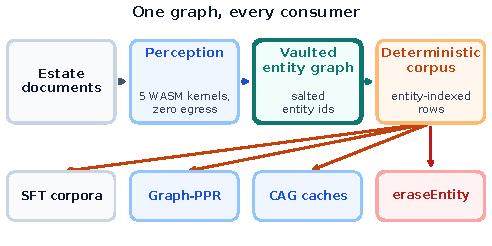
\includegraphics[width=\columnwidth]{figs/fig_k7_architecture.pdf}
\caption{The architecture. Five zero-import WASM kernels perceive the estate's documents with zero egress; every detected value is vaulted behind a salted placeholder and derives a stable entity identifier, so the corpus and its entity index form one resolved graph with per-sample provenance and conformal certificates. The same graph grounds every downstream consumer: the training corpora (per-block, composed, identity-pair; vaulted or readable views), question-time Graph-PPR retrieval, the CAG caches (fixed set-cover prefill and the per-question identity-keyed hybrid, both prefilling the model's key-value cache), and \texttt{eraseEntity}, which regenerates the corpus minus one entity because the graph names exactly the samples and spans an entity owns.}
\label{fig:architecture}
\end{figure}

Figure~\ref{fig:architecture} shows the whole path from estate documents to the consumers the downstream comparison measures. The data model everything sits on is small: every detected value is vaulted behind a salted placeholder and derives a stable entity identifier (an HMAC of the workspace salt over the value's class and canonical form), every sample records the identifiers it mentions, the entity index records every sample an entity touches, and the corpus is a pure function of (inputs, view, engine version). The same resolved graph then grounds every consumer without rebuilding identity for any of them: the per-block and composed training corpora are traversals of it (Section~\ref{sec:composition}); Graph-PPR retrieval runs personalized PageRank~\cite{haveliwala2002topic} over it at question time; the CAG arms select composed records through it (a fixed set-cover cache, and the per-question hybrid keyed by the asked person's canonical identity) and prefill the model's key-value cache with them; and \texttt{eraseEntity} regenerates the corpus minus one entity because the graph names exactly which samples and spans an entity owns (Section~\ref{sec:erasure}). Positional chunking resolves none of this: its samples carry no identity, so each consumer would have to rebuild identity separately or go without it, and erasure has no index to name the bytes to remove. Which consumer pays off, and by how much, is what the head-to-head of Section~\ref{sec:headtohead} measures.

Three properties of the corpus follow from the seam design:

\begin{itemize}
  \item \textbf{Determinism.} The corpus is a pure function of (inputs, view, engine version): no timestamps, no unseeded randomness, fixed key order, content-digest sample IDs and ordering. A receipt pins the corpus SHA-256 and the engine-version hash, so kernel or source drift invalidates rather than silently corrupts.
  \item \textbf{Entity indexing.} Every sample records the entity identifiers it mentions; the entity index records every sample an entity touches. A ground-truth person (name, email, phone) is three values and therefore three vault identifiers; the corpus indexes each value, and cross-modal spoken-form variants resolve onto the same salted identifiers.
  \item \textbf{Certificates.} Each sample is re-scanned after masking; any residual scanner hit that is not a vault placeholder counts against the sample. The per-sample certificate is the conformal gate's decision with a certified binomial recall bound (Clopper--Pearson~\cite{clopper1934binomial}, fixed-sequence Learn-Then-Test~\cite{angelopoulos2021ltt} over the shipped binomial CDF kernel).
\end{itemize}

\section{The Sample Schema}
\label{sec:schema}

A training sample in the exported JSONL is:

\begin{itemize}
  \item \texttt{id}: SHA-256 content digest over source, byte-range (or a derived-format marker), and text; byte-range collisions fail loudly as engine bugs, and benign repeated derived-format content (a quoted line, two same-titled slides) disambiguates deterministically.
  \item \texttt{source}, \texttt{sourceRange}: provenance, the input name and, on plain-byte surfaces (txt/csv/sql), exact byte ranges into the source. Derived formats (eml/pptx/vtt/wav) reflow text, so those blocks carry no byte range, and the schema marks them as derived-format in the sample id.
  \item \texttt{entities}: the vault-salted entity identifiers the sample mentions. In the per-block export this field is JSONL metadata; the training loss sees identity only where a view renders it into tokens (the composed corpus names its target entity, and the identity-pair set renders ids as the SFT answer).
  \item \texttt{messages}: the SFT turn structure (system prompt, user task, masked assistant content), with placeholder masking so the retrain recipe can mask loss on vault spans.
\end{itemize}

Per-sample certificates ride in the run artifact keyed by the same content-digest ID (adding fields to the JSONL lines would change the frozen corpus SHA-256 receipts, so the seam bytes are reused untouched).

The same seam exposes two declarative view dimensions on top of this schema. \texttt{identity}: the \texttt{vaulted} default described above, or an explicit \texttt{readable} opt-in for the user training a model on their own documents who wants it to learn real names: unmasked content and canonical readable entity anchors. In the readable view the certificate ceremony does not run, so the conformal bound is a property of the vaulted default only. The operator is accountable for the lawful basis of the opt-in. The readable export carries no certificates. Erasure of a readable-derived adapter follows the retrain path, not corpus regeneration. The vaulted machinery is not a tier or an upsell; it is simply how the engine runs by default. \texttt{composition}: the per-block corpus above, or the composed corpus of Section~\ref{sec:composition}. Both dimensions are deterministic pure functions of (inputs, view, engine version), erasure is span-exact in every view, and the view is recorded in the receipt. Which claim lives where matters: in the vaulted default the retrain recipe masks loss on vault spans, so the adapter learns structure, not who anyone is; the standalone-knowledge \emph{training} benefit, if it exists, lives in the readable view, and the designed comparison of Section~\ref{sec:claims} therefore runs readable by default. The vaulted default's own claim is lineage and exact erasure, not learned names.

\section{Measured Receipts}
\label{sec:measurements}

All numbers in this section are computed from checked-in artifacts by a CI check; none are hand-tuned. A receipt is a hash-pinned artifact field: a corpus SHA-256, an engine-version hash, or a diff receipt. The test estate is deterministic (recorded seed), 12 files across 4 departments (IT, business, shared, meetings) and 8 modalities, with 24 ground-truth entities, 16 people, 4 organizational IDs, 4 project codenames, each appearing in at least two departments and two modalities. Ground truth lives only in the generator manifest; the engine never receives it.

\paragraph{Artifact availability.}
Every number in this paper is emitted by a checked-in runner in the project repository (\url{https://github.com/gegearsyah/versieve}) at commit \texttt{1e35603}. The result JSON files carry the corpus SHA-256, the engine-version SHA-256, and the seed. The five kernels total $388{,}797$\,B: \texttt{versieve\_clean.wasm} ($14{,}633$\,B), \texttt{versieve\_graph.wasm} ($54{,}402$\,B), \texttt{versieve\_dl.wasm} ($60{,}096$\,B), \texttt{versieve\_sql.wasm} ($55{,}635$\,B), and \texttt{versieve\_media.wasm} ($204{,}031$\,B); their SHA-256 prefixes are \texttt{5cb584ed} (clean), \texttt{3313ab50} (graph), \texttt{2ff6e775} (dl), \texttt{45cdead8} (sql), and \texttt{c4758922} (media); the full digests are reproducible with \texttt{sha256sum vendor/wasm/*.wasm} at that commit. The training checkpoint is \texttt{Qwen/Qwen2.5-1.5B-Instruct}; the judges are Qwen2.5-7B-Instruct and Llama-3.2-3B-Instruct.

\paragraph{Extraction fidelity.}
Table~\ref{tab:argon} reports the perception benchmark over six ground-truth-by-construction workspaces. These are \emph{construction-validation} numbers: the fixtures are synthetic, and the engine recovers what its own fixture corpus encodes (chart series, diagram topology, speaker turns, deictic bindings, and SQL aggregations) where a flat-text baseline recovers none of it. The flat-text baseline scores 0 by construction on the modalities it cannot express, so the table is construction validation, not an extractor comparison; a comparison against real extraction pipelines is open work.

\begin{table}[t]
\centering
\caption{Perception benchmark (six synthetic workspaces, oracle = ground truth by construction). Flat-text baseline cannot express chart inversion, diagram topology, SQL, diarization, or deictic binding; its conventional values are documented beside each metric in the artifact. Workspace 4's representation is keyframes + WAV + VTT: no video-decode claim. $\dagger$~None recovered.}
\label{tab:argon}
\scriptsize
\setlength{\tabcolsep}{3pt}
\begin{tabular}{llrr}
\toprule
Workspace & Metric & Baseline & Versieve \\
\midrule
W1 deck (.pptx) & diagram-edge F1 (\%) & 0 & 100 \\
 & chart-series match (\%) & 0 & 100 \\
W2 raster (.png) & chart mean RelErr (\%) & 100$^{\dagger}$ & 0.0187 \\
 & points within 2\% RelErr (\%) & 0 & 100 \\
 & diagram-edge F1 (\%) & 0 & 100 \\
W3 audio (.wav) & speaker purity (\%) & 55.56 & 100 \\
 & prosodic-intent acc. (\%) & 44.44 & 100 \\
W4 keyf.+WAV+VTT & deictic grounding recall (\%) & 0 & 100 \\
W5 tables (.xlsx/.pdf) & SQL exact-match (\%) & 0 & 100 \\
W6 bundle & cross-modal link (\%) & 0 & 100 \\
 & multi-hop QA (\%) & 0 & 100 \\
\bottomrule
\end{tabular}
\end{table}

\paragraph{Detection and certificates.}
Over the estate, the scanner detects with zero misses: PERSON $153$, EMAIL $57$, PHONE $28$, DATE\_OF\_BIRTH $20$, ADDRESS $3$, and one injected GITHUB\_PAT, which marks its sample \texttt{QUARANTINE\_SECRET} by design: the sample ships with that mark and fails its certificate, while every other sample's certificate must pass. Organizational IDs and project codenames have no engine detector class; they are estate ground truth only, and no coverage is claimed for them. The per-sample certificate pass rate is $95.8333\%$ (23 of 24 samples), with a certified lower bound of $81.7108\%$ at the stated $95\%$ confidence. All bounds are one-sided 95\% Clopper--Pearson bounds. The certified lower bound of $81.7108\%$ is the one-sided bound on $23/24$ (the two-sided bound is $78.88\%$); the per-class bounds assume zero detected misses against manifest ground truth. The certificate is detector-closed: it re-scans with the same detector family that performed the masking, so it certifies absence of PII detectable by this scanner, not absence to an independent auditor; and with 24 samples the lower bound is small-sample arithmetic, not evidence. Per-class certified recall lower bounds degrade with class rarity: PERSON $98.06\%$ over $153$ detections, EMAIL $94.88\%$ over $57$, PHONE $89.85\%$ over $28$, DATE\_OF\_BIRTH $86.09\%$ over $20$, ADDRESS $36.84\%$ over $3$, and the quarantined GITHUB\_PAT class $5\%$ over its single detection.

\paragraph{Cross-department linking.}
The manifest's ground truth defines 54 (entity, department-pair) cross-department links on the IT and business sides, the two departments the linking check covers; the pipeline recovers all 54 with zero false positives (precision, recall, and F1 at $100\%$ at that unit), and all 16 ground-truth people resolve to the same vault identifiers across those two departments. The emitted connection graph has 92 nodes and 208 edges over the masked corpus, SHA-pinned in the artifact. This is the standalone-knowledge property measured: records in different departments, in different modalities, about the same person, carry the same identity into training. The unit linked is the value, not the person: a person's name, email, and phone carry separate identifiers, and 54/54 recovery at this unit is exact matching on planted values. Noise-tolerant resolution (nicknames, shared inboxes, same-name collisions, stale records), scored with pairwise and B-cubed~\cite{bagga1998bcubed} precision and recall including false-merge rate, is the open measurement of the benchmark line: the noisy estate built for it (Section~\ref{sec:headtohead}) drops the trivial exact-match baseline to a $24.27\%$ pairwise recall floor, and the openly licensed second estate of Section~\ref{sec:openestate} holds the same machinery under a $61.46\%$ floor on real meeting text. The estate's own PPRL benchmark~\cite{christen2012datamatching} measures a $4.88\%$ false-link rate at its dev threshold on a 500-common-names collision set: a designed-collision stress reading, not a representative rate for real estates.

\paragraph{Erasure.}
The corpus indexes $76$ engine entities while the manifest holds $24$ ground-truth entities: ground-truth entities are canonical, so a person is one entity across name, email, and phone, whereas the corpus indexes each distinct detected value as its own salted engine entity. Deletion requests over 1\%, 5\%, and 20\% of the 76 indexed entities select disjoint slices by a seeded shuffle; each request regenerates the corpus, and the byte-diff against the original is verified to be exactly the erased entities' spans: token bytes in content plus the entity-ID entries in the per-sample lists. All three fractions verify exact, with unchanged samples byte-identical (Table~\ref{tab:erasure}).

\begin{table}[t]
\centering
\caption{Amnesiac Corpus ablation (CPU side; the 24-sample, 76-entity corpus). ``Measured delta'' includes token spans plus entity-id list entries, the full erased footprint per the diff receipts. 23 of the 24 samples carry a passing certificate; the quarantined 24th is the injected-secret sample.}
\label{tab:erasure}
\scriptsize
\begin{tabular}{lrrr}
\toprule
Deletion fraction & Entities erased & Token span bytes & Measured delta \\
\midrule
1\% & 1 & 24\,B & $-51$\,B \\
5\% & 4 & 71\,B & $-217$\,B \\
20\% & 15 & 999\,B & $-2406$\,B \\
\bottomrule
\end{tabular}
\end{table}

\section{Relational Composition}
\label{sec:composition}

The composed corpus is emitted by the same builder under a versioned composition policy (receipted as \texttt{composed-v1}). For each resolved entity, one SFT sample renders all of that entity's evidence blocks as labeled \texttt{[source]} segments in canonical order (byte-ranged blocks first, ordered by source name and byte offset, then derived-format blocks) under a fixed per-entity block cap, so high-degree entities cannot flood the corpus with near-duplicate renders. Every composed sample names its target entity and carries a provenance array enumerating each contributing document and its range.

Three receipts hold today and are asserted in CI. \emph{Determinism}: two composed builds over the same inputs are byte-identical. \emph{Erasure re-proven on the composed corpus, not inherited}: erasing the entity a composed sample exists to render retracts that sample from the corpus, while erasing a co-mentioned entity removes exactly that entity's spans from the render; and a build-failing guard asserts that the two internal derivations of the same composed erasure agree byte-for-byte, so a subtle divergence fails the build instead of shipping. \emph{Regression}: the default per-block corpus is untouched by the composition code path; its pinned corpus SHA-256 reproduces.

Whether an adapter trained on composed samples beats, matches, or loses to per-block, flat-chunked, or retrieval baselines is the head-to-head of Section~\ref{sec:headtohead}, and composition carries two measured costs alongside its benefit: the false-merge amplification and hub duplication of Section~\ref{sec:failuremodes}.

\subsection{Failure Modes, Measured}
\label{sec:failuremodes}

Composition ships with two costs the per-block corpus does not carry, and both are measured on the noisy estate rather than designed.

\paragraph{False-merge amplification.}
Inducing controlled false merges over a ladder of merge rates (the 20 designed collision pairs always merged, plus a seeded prefix of disjoint random pairs, 0 to 72 merged person classes) and measuring corruption as person occurrences carried in a record that mixes two real people under one identity: at a $25\%$ merge rate the composed corpus corrupts $0.3214$ of its world-mappable occurrences against $0.0224$ for per-block, an amplification factor of $14.32$ (raw fractions $0.321364$ and $0.022442$); at $50\%$ the rates are $0.5512$ against $0.0431$, a factor of $12.79$. At the two lowest rates ($5\%$ and $10\%$) per-block corruption is exactly zero while composed already sits at $0.1329$ and $0.1786$; no amplification factor is defined where the per-block rate is zero. Per-block is not undamaged: every falsely merged mention is attributed to a false identity in both views ($148$ to $614$ occurrences across the ladder); composition's additional damage is that one record renders both people under one canonical anchor, and all 72 merged classes produce such a false-name anchor at the top rate.

\paragraph{Hub duplication.}
MinHash near-duplicate analysis~\cite{broder1997resemblance} of the composed corpus (16-character shingles, 128 hash functions, 32 bands of 4 rows, candidate pairs confirmed by exact shingle Jaccard $\geq 0.8$): the failure-mode build carries $1{,}113$ samples (corpus SHA-256 prefix \texttt{9290b008}) and the equal-budget training arm's receipt records $1{,}106$ samples (corpus SHA-256 prefix \texttt{32fa477f}); these are two receipted builds of the same composition policy, and no claim in this paper compares counts across the two builds. The failure-mode build yields $20{,}627$ near-duplicate pairs of which $12{,}569$ are exact duplicates, and every composed sample sits in a near-duplicate pair (fraction $1.0$). Corpus-level duplication is documented to amplify verbatim memorization in language models~\cite{lee2022dedup}, so this near-duplicate structure is a memorization risk and not only a storage artifact. The mechanism is co-mention block reuse: one evidence block renders inside the record of every co-mentioning entity, so the corpus repeats its own source bytes. The six samples truncated by the hub cap are the near-duplicate-free ones, so the cap policy is not the cause; co-mention is. The degree-versus-benefit saturation curve (whether a $k$-degree entity's record still helps at $k \geq 8$) stays designed-not-run, recorded in the artifact with its full design.

\section{The Head-to-Head, Measured}
\label{sec:headtohead}

The comparison this artifact was built for: eleven arms on the same estate, one token budget per arm capped at $25{,}755$ training tokens, one recipe, exact-match scoring against manifest truth, and two blinded judges for the arms scored under the judge protocol.

\paragraph{The estate.}
The noisy estate is deterministic (seed 20261124): $115$ documents over five text modalities (rosters in CSV and SQL, memos, chat logs, meeting captions), $250$ people, $2{,}368$ person mentions, and the eight designed noise types of the committed estate spec (\texttt{docs/2026-11-24-noisy-estate-}\allowbreak\texttt{benchmark-spec.md}) (typos and OCR damage, nicknames, initials, case and format variants, shared inboxes, 20 same-name collision pairs, stale records, cross-document disagreement). The trivial exact-match baseline over identically normalized mention surfaces scores pairwise recall $24.27\%$ at precision $91.83\%$ with $257$ false merges, every one on the designed collision pairs; the binding gate (recall under $90\%$ plus at least one collision false merge) passes, so the estate is a benchmark and not a solved key. Sixty eval questions live only in the manifest: $24$ single-document (Q1), $24$ cross-document (Q2), and $12$ disambiguation questions between same-name people (Q3). The engine and every training corpus see only the estate documents; the questions, answers, and truth never enter any arm's training data.

\paragraph{The design.}
Five trained arms at one token budget capped at $25{,}755$ training tokens each (prompt plus target after the assistant-loss render): flat 800-character windows in document order; the per-block readable corpus; the composed corpus; the composed corpus plus identity-contrastive pairs; and the per-block vaulted corpus, the privacy-cost ablation of the per-block arm. The cap is enforced by deterministic head truncation in corpus file order (hash-id order, blind to ground truth): rows are appended until the next row would exceed the cap, so realized totals sit at or just below it (flat $25{,}724$, per-block $25{,}740$, composed $25{,}088$, composed-plus-pairs $25{,}565$, vaulted $25{,}755$ tokens) and kept-row counts differ sharply by format: flat keeps $100$ of $178$ rows, per-block $194$ of $216$, composed $41$ of $1{,}106$ ($3.7\%$; a separate receipted build of the failure-mode corpus of Section~\ref{sec:failuremodes}), composed-plus-pairs $50$ of $3{,}322$, and vaulted all $216$; composed keeps $908$ distinct entities against per-block's $1{,}029$ (flat carries no entity list by construction). Coverage is therefore part of what the equal-budget protocol measures: composed rows are larger and span more entities, so the same cap keeps fewer, broader records, and the composed-over-per-block ordering is an ordering under this truncation regime, not a property of the formats independent of it. Two arms train nothing: Graph-PPR retrieval (personalized PageRank over the same entity graph, top-6 contexts fed to the untrained base model at question time) and the base model alone. The recipe is sealed, meaning fixed before the head-to-head ran, from a prior 18-combination epoch and learning-rate sweep; the sweep belongs to the companion local-training study~\cite{ardiyansyah2026localtraining}, and it selected on that study's compliance QA, not on the 60 manifest questions used here. Qwen2.5-1.5B-Instruct, LoRA rank 16, $\alpha$ 32, 160 steps, learning rate $2 \times 10^{-4}$; a 104-row canary batch (12 canaries at 1, 5, and 20 repetitions) is appended identically to every trained arm, so canary exposure is comparable across arms. Answers are scored by exact match against manifest values for every arm; two blinded judges that never see the arm identity (a strict Qwen2.5-7B judge and a cross-family generous Llama-3.2-3B judge) score the trained arms and the Graph-PPR and base controls, whose row agreement ($6.7$ to $41.7\%$ across arms) is recorded because the judges disagree and neither is cherry-picked. Such sensitivity is documented: LLM judges carry positional, verbosity, and self-preference biases~\cite{zheng2023judging}, and their rankings can be manipulated by changing response order~\cite{wang2023fair}.

\begin{table}[t]
\centering
\caption{Closed-book exact match ($\%$) on the noisy estate's 60 manifest questions by stratum (Q1 single-document, $n{=}24$; Q2 cross-document, $n{=}24$; Q3 disambiguation, $n{=}12$), with mean judge scores on a 0-to-2 scale across the two judges. Trained arms share one $25{,}755$-token budget and one recipe and are head-truncated in corpus order to the shared cap; kept rows per arm: flat $100/178$, per-block $194/216$, composed $41/1{,}106$, composed-plus-pairs $50/3{,}322$, vaulted $216/216$. BM25, fixed-cache CAG, and the per-question hybrid routing arms train nothing; as a design choice they are scored by exact match only, with no judges run at scoring time, on the same estate, rows, and base model as the other arms (Scored column: EM$+$J means exact match plus the two blinded judges, EM means exact match only), so the judge columns are comparable only within the EM$+$J rows and no cross-protocol judge analysis is made. $^{\ast}$The CAG set-cover arm is an evaluation-informed upper bound: its cache contents are optimized against the question population itself, which deployment cannot do. \texttt{CAG hybrid routing} ($81.7\%$) is a conditional upper bound given oracle manifest identity; \texttt{Engine-resolved router} (\texttt{retrieval\_engine}, $68.3\%$) is the measured end-to-end router over engine-produced \texttt{buildAmnesiacCorpus} entity identifiers, scored under EM$+$J.}
\label{tab:k3}
\scriptsize
\setlength{\tabcolsep}{3pt}
\begin{tabular}{lrrrrrrl}
\toprule
Arm & Q1 & Q2 & Q3 & All & Judge & Llama & Scored \\
\midrule
Flat 800-char chunks & 4.2 & 8.3 & 8.3 & 6.7 & 0.20 & 1.05 & EM$+$J \\
Per-block (readable) & 8.3 & 12.5 & 8.3 & 10.0 & 0.23 & 0.90 & EM$+$J \\
Composed & 8.3 & 12.5 & 16.7 & 11.7 & 0.23 & 0.92 & EM$+$J \\
Composed + pairs & 4.2 & 0.0 & 0.0 & 1.7 & 0.03 & 0.77 & EM$+$J \\
Per-block (vaulted) & 4.2 & 0.0 & 0.0 & 1.7 & 0.07 & 0.82 & EM$+$J \\
Graph-PPR retrieval & 41.7 & 83.3 & 16.7 & 53.3 & 1.05 & 1.37 & EM$+$J \\
Base (no fine-tune) & 4.2 & 0.0 & 0.0 & 1.7 & 0.03 & 0.98 & EM$+$J \\
BM25 retrieval & 58.3 & 87.5 & 8.3 & 60.0 & -- & -- & EM \\
CAG set-cover$^{\ast}$ & 37.5 & 75.0 & 33.3 & 51.7 & -- & -- & EM \\
CAG hybrid routing & 87.5 & 79.2 & 75.0 & 81.7 & -- & -- & EM \\
Engine-resolved router & 83.3 & 62.5 & 50.0 & 68.3 & 1.33 & 1.47 & EM$+$J \\
\bottomrule
\end{tabular}
\end{table}

\paragraph{The reading.}
Four results carry weight. First, the graph pays off as a retrieval index, not as a training format, at this scale: retrieval with no fine-tuning answers $53.3\%$ exactly, $4.6$ times the composed arm's $11.7\%$, and $83.3\%$ on the cross-document stratum the composition policy was designed for, because the contexts it retrieves already join the documents the trained arms must bake into weights. The win is a retrieval result, not a long-context result: it supplies six retrieved contexts to a 1.5B base, below the regime in which long-context answering has been reported to match or exceed retrieval~\cite{li2024raglc}. Second, the trained formats do not separate: composed ($11.7\%$), per-block ($10.0\%$), and flat ($6.7\%$) sit within a margin that no McNemar comparison separates, composed against per-block is $p{=}1.00$ and composed against base is $p{=}0.07$, so this study makes no trained-format claim. The point difference lands on the 12-question disambiguation stratum ($16.7\%$ against $8.3\%$): one question of twelve. The margins are small, 60 questions make every cell a handful of items, and this is one run at one starved budget. Third, the composed-plus-pairs arm failed by mechanism, not by verdict on the pair idea: under the shared budget the pair rows displaced composed rows until only $50$ rows with $9{,}947$ learnable tokens survived (against $41$ rows and $23{,}608$ learnable tokens for composed alone), and the arm scores exactly base. Fourth, the vaulted ablation scores base on closed-book identity questions ($1.7\%$) because the vault masks $36.31\%$ of subwords: the identity the questions ask about was never in the learnable text. The arm is a construction-consistency check: a privacy-cost measurement would need a utility battery indifferent to identity, and none is run here. The readable opt-in seam exists for the user training a model on their own documents.

\paragraph{Non-training controls.}
Three further arms train nothing and were scored by exact match only, with no judges run, on the same estate, rows, and base model as the other seven arms. A from-scratch BM25 retriever over the same passage pool (Okapi BM25~\cite{robertson2009bm25}, $k_1{=}1.5$, $b{=}0.75$, $216$ passages reconstructed from the raw estate bytes), feeding top-6 contexts to the base model, answers $60.0\%$ overall ($58.3\%$ Q1, $87.5\%$ Q2, $8.3\%$ Q3), numerically above the graph retriever's $53.3\%$ and within noise at $n{=}60$; on this estate the graph's contribution is not retrieval quality. The per-stratum counts show a direction rather than an inferential claim, at stratum sizes of $24$, $24$, and $12$: BM25 answers $1$ of $12$ disambiguation questions correctly, Graph-PPR $2$ of $12$, the cache arm $4$ of $12$, and the hybrid routing arm $9$ of $12$. Cache-augmented generation over the composed records prefills the cache once, $8$ composed per-entity records selected by greedy set-cover over the $52$ unique question persons and $16{,}607$ prefill tokens, slightly below the $21$k-to-$85$k corpus-size regime the CAG literature evaluates~\cite{chan2024cag}; the set-cover optimizes the cache contents against the question population itself, which deployment cannot do, so this arm is an evaluation-informed upper bound for fixed-cache CAG (marked in Table~\ref{tab:k3}). It ties the retrieval arms overall, within noise at $n{=}60$ ($51.7\%$ against $53.3\%$ and $60.0\%$), leads on disambiguation ($33.3\%$, $4$ of $12$), and trails on single-document questions ($37.5\%$ against BM25's $58.3\%$). The token accounting is the amortization: each question appends $15$ mean tokens after the one-time prefill, against $1{,}004$ mean prompt tokens per question for the retrieval arms. The mechanism is visible in the strata: a fixed cache cannot fetch the one document that holds the answer, while the composed records carry enough cross-document context to help the collision questions. A third arm measures the per-question selection this suggests. It is not the hybrid design the CAG literature itself proposes (a preloaded core plus retrieval for edge cases)~\cite{chan2024cag}: it selects by identity with no retrieval fallback. Per question, the records whose own target carries the asked person's canonical identity key (the person's $2$ or $3$ subject records) are prefilled as a fresh cache, and the question is appended to it. It answers $81.7\%$ overall ($87.5\%$ Q1, $79.2\%$ Q2, $75.0\%$ Q3, $9$ of $12$ disambiguation), the routing upper bound in the table; at $n{=}60$ this is one estate's measurement. Its router receives the question's resolved person identity instead of doing retrieval, so disambiguation is settled by routing rather than in context; in deployment that resolution is the identity graph's own task and the questions state the full name, but the arm scores routing given a correct resolution, not resolution itself. $81.7\%$ is therefore a conditional upper bound on the routing arm given oracle identity, not a deployment measurement. The gain gives up the amortization: a mean of $2{,}940$ prefill tokens rebuilds the cache per question, against the fixed cache's one-time $16{,}607$-token prefill, though each question still appends only $15$ mean tokens. A fourth non-training arm (\texttt{retrieval\_engine}, labeled \texttt{Engine-resolved router} in Table~\ref{tab:k3}) measures end-to-end routing on the engine's own \texttt{buildAmnesiacCorpus} entity identifiers with zero manifest access: matching the question string at alphanumeric word boundaries against engine target identifiers selects one composed subject record per question ($1{,}210.8$ mean context tokens, $1{,}280.1$ mean prompt tokens under the shared $31{,}744$-token cap) and answers $68.3\%$ overall ($83.3\%$ Q1, $62.5\%$ Q2, $50.0\%$ Q3, $6$ of $12$ disambiguation; strict Qwen2.5-7B judge mean $1.33$, cross-family Llama-3.2-3B judge mean $1.47$, row agreement $53.3\%$). The $-13.3$-percentage-point gap below the $81.7\%$ conditional upper bound quantifies the resolution gap when the engine indexes name, email, and phone as separate entities and merges same-name collision pairs under one \texttt{ent:person} target. Cache invalidation at erasure granularity follows from the byte-diff receipts the corpus machinery already produces, a mechanism this measurement does not benchmark.

\paragraph{Uncertainty at $n{=}60$.}
Every exact-match percentage in Table~\ref{tab:k3} carries an exact binomial (Clopper--Pearson) $95\%$ interval, and at $n{=}60$ those intervals are wide: Graph-PPR $53.3\%$ ($40.0$ to $66.3$), BM25 $60.0\%$ ($46.5$ to $72.4$), CAG $51.7\%$ ($38.4$ to $64.8$), hybrid routing $81.7\%$ ($69.6$ to $90.5$; routing given a correctly resolved identity), composed $11.7\%$ ($4.8$ to $22.6$), per-block $10.0\%$ ($3.8$ to $20.5$), flat $6.7\%$ ($1.8$ to $16.2$), and base $1.7\%$ ($0.0$ to $8.9$). Interval overlap decides nothing in either direction. The 60 questions are a fixed authored set, the entire frame, written into the manifest before any arm ran; they are not a sample from a question population, and the intervals quantify per-question answer variability on this fixed set, not sampling error. Because all ten arms answer the same 60 questions, every pairwise comparison is paired, and the decisive test is exact McNemar over the committed per-question rows, Holm-corrected within each claim's comparison family at $\alpha{=}0.05$: the family of the hybrid arm against the other three non-training arms, the family of the trained formats against one another and the base, the family of the retrieval and fixed-cache arms against one another, and the twenty retrieval-or-cache-versus-trained comparisons; every $p$ is recomputed by the CI checker from the rows. After correction: the hybrid routing arm separates from CAG (raw $p{=}0.0001$, adjusted $0.0004$), from Graph-PPR (raw $0.0023$, adjusted $0.0046$), and from BM25 (raw $0.0146$, adjusted $0.0146$); every retrieval or cache arm separates from every trained arm (adjusted $p < 10^{-4}$); no trained-format comparison separates (composed against per-block $p{=}1.00$, composed against flat $0.55$, per-block against flat $0.73$, composed against base $0.07$, per-block against base $0.13$, none surviving correction); and the retrieval and fixed-cache arms do not separate from one another (BM25 against Graph-PPR $0.39$, CAG against Graph-PPR $1.00$, CAG against BM25 $0.49$). For the measured end-to-end \texttt{retrieval\_engine} router, the Clopper--Pearson $95\%$ interval is $68.3\%$ ($55.0$ to $79.7$ overall; $62.6$ to $95.3$ Q1, $40.6$ to $81.2$ Q2, $21.1$ to $78.9$ Q3): it trails the $81.7\%$ oracle bound at raw McNemar $p{=}0.0386$ (paired permutation $p{=}0.0340$, Holm-adjusted $p{=}0.1543$ across the four non-training comparators), does not separate statistically at $n{=}60$ from BM25 (raw McNemar $p{=}0.4421$, permutation $p{=}0.4288$), Graph-PPR (raw $p{=}0.1360$, permutation $p{=}0.1329$), or fixed-cache CAG (raw $p{=}0.0525$, permutation $p{=}0.0475$), and separates from every trained arm and base (Holm-adjusted McNemar $p < 10^{-4}$, permutation $p{=}0.0005$).

\paragraph{Canary exposure and fluency.}
The canary batch is 12 planted canaries (email, phone, and name types) at 1, 5, and 20 repetitions, appended identically to every trained arm, scored by Carlini-style rank-based exposure in bits~\cite{carlini_secret_sharer}. Exposure is flat across trained arms ($8.48$ to $8.57$ bits over the 12 canaries, against $4.25$ bits for the untrained base, so fine-tuning roughly doubles canary exposure at every trained arm), and the rank-1 count agrees: every trained arm ranks $8$ of the $12$ canaries first, the base $3$ of $12$, and the base's rank-1 canaries are the three name canaries, the type an instruct model already knows. LoRA adapters can retain planted secrets depending on adapter placement and repetition~\cite{tan_lora_memorization}; what the flat exposure says is that the training-format choice does not move memorization at this scale. Held-out perplexity is measured on 10 fixed generic paragraphs ($380$ tokens, no estate content): every trained arm loses fluency against base ($26.1$), composed moves to $32.5$, and vaulted is worst at $43.9$, with zero placeholder emissions. The regime is capacity-starved by design: a 1.5B adapter, 160 steps, $25{,}755$ tokens, each estate fact appearing in one or two documents, where knowledge-capacity results~\cite{allenzhu2024knowledge} predict that facts seen in few varied forms are barely extractable. Whether the composed-over-flat ordering grows, holds, or inverts at larger budgets is open work; the retrieval arm's win is the one result with no training-budget dependence.

\section{External Validity: A Second Estate from Openly Licensed Data}
\label{sec:openestate}

\paragraph{A layered estate, never mixed.}
The noisy estate is synthetic. The second estate is built from openly licensed real data under one rule: real identity and overlay identity are scored in separate layers, and no metric mixes them. Layer R is real: 12 meeting transcripts from AMI and ICSI as distributed by QMSum (MIT repackaging; the underlying corpus is CC BY 4.0), truth = the corpus's own speaker labels, plus six pinned AMI Mix-Headset recordings (CC BY 4.0, per-file SHA-256 pins) whose 62 corpus-labeled people are keyed exactly as the corpus distributes them; overlay never touches audio. Layer O plants a 60-person overlay cast over real transcript text with the same eight noise types as the noisy estate, truth by construction. Every fixture is committed as data with its license recorded in the manifest.

\paragraph{The floor on real data.}
The same trivial exact-match machinery, applied per layer. Layer O: pairwise recall $61.46\%$, precision $76.10\%$, and $2{,}303$ false merges, every one on the 12 designed collision pairs; the binding gate passes, so overlay identity over real text is a benchmark and not a solved key. Layer R is reported as-is and ungated: recall $100\%$ at precision $22.79\%$, because exact-match transitive closure merges every verbatim-repeating surface: the corpus's role labels repeat verbatim across meetings, so distinct speakers sharing a label string collapse into one group ($7{,}449$ mentions into $21$ string groups, $2{,}037{,}812$ false merges, none on designed collision pairs); that number is a calibration floor, not an engine score. As a third, conditional slice, an Enron email subset (no stated license; benchmarked on the authors' machine only, with zero Enron bytes in this repository and aggregates plus an archive SHA-256 pin recorded in the artifact) floors at pairwise recall $26.60\%$ and precision $82.06\%$, with $273$ false merges of which $260$ fall on designed collision pairs. These numbers are floors for engine claims on real data, not engine claims: identity resolution on this estate is the open resolution-scoring measurement.

\section{The Erasure Property}
\label{sec:erasure}

Whether erasure under GDPR Article~17~\cite{gdpr_art17} must extend to models trained on the erased data is a regulatory question this artifact does not settle; what it supplies is the evidence a settlement would need, in two halves:

\begin{itemize}
  \item \textbf{Corpus half (measured above).} \texttt{eraseEntity} regenerates the corpus minus one entity with a diff receipt: changed samples, removed span count and bytes, corpus SHA-256 before and after, and a failure that throws, loudly, whenever the byte-diff exceeds the erased entity's spans. Receipts are version-pinned: an engine-version drift invalidates regeneration instead of silently producing different bytes. Erasure is corpus-side: the regenerated corpus, the entity-index row, and the diff receipt are the receipt's full scope. The vault holds no raw values (entity identifiers are salted HMAC derivations; raw values live only in the source inputs, which erasure does not touch), but vault entries and the workspace salt are retained so non-erased entities keep stable identifiers; whether a deployment must also purge its source inputs and vault entries is deployment policy outside this receipt.
  \item \textbf{Adapter half (pending GPU backfill).} The export ships a sealed, seeded LoRA retrain recipe (rank 16, $\alpha$ 32, fixed steps and learning rate, placeholder-masked loss on vault spans); erasure completes by retraining the adapter over the regenerated corpus. The three GPU-dependent measurements (retrain wall-clock versus full retrain from scratch, a head-to-head against SISA on the same estate, and Carlini canary exposure~\cite{carlini_secret_sharer} pre- versus post-retrain against the chance rate) are structured in the artifact as \texttt{pending-gpu} and are not reported in this paper.
\end{itemize}

\paragraph{Salt lifecycle.}
The operator holds the workspace salt. Salt compromise permits offline confirmation of guessed low-entropy values; different salts make the same value unlinkable across workspaces. Rotating the salt changes every identifier and therefore invalidates stored receipts unless receipts are versioned against the salt.

\paragraph{Deployment costs.}
An operator runs per-sample certificate computation at build time and holds custody of the vault and the workspace salt; a data subject can receive the erasure receipt for their entity; third-party verification is a re-run of the pinned build against the recorded corpus hash.

\section{What This Paper Does Not Claim}
\label{sec:claims}

The gatekeeper certificate bounds residual detectable PII at a stated confidence, is detector-closed, and is small-sample (Section~\ref{sec:measurements}); it is a build-time check over corpus bytes, not a property of a trained model and not an audit. The people the corpus describes, whom the vaulted default exists to protect, hold the erasure receipt as their recourse. CLIOPATRA- and LeakageBench-class results are why redaction is not promoted to a privacy guarantee here.

The perception and linking numbers are construction-validation on synthetic, ground-truth-by-construction fixtures. They prove the pipeline does what it is constructed to do on data whose truth is known; they do not predict open-world accuracy. The second estate (Section~\ref{sec:openestate}) validates the floor machinery on openly licensed real data, not the engine.

The motivating hypothesis, that training on graph-grounded, standalone-knowledge samples beats training on positionally stitched chunks, is measured in Section~\ref{sec:headtohead}: composed ($11.7\%$) and per-block ($10.0\%$) do not separate at $n{=}60$ (McNemar $p{=}1.00$), composed versus base is $p{=}0.07$, and no trained-format comparison separates; the whole point difference between the two formats is one question on the 12-question disambiguation stratum. The same entity graph used as a retrieval index with no fine-tuning answers $53.3\%$, $4.6$ times the composed arm's $11.7\%$. The boundaries of that measurement are the claim: one 1.5B-parameter adapter, 160 steps, a $25{,}755$-token budget, and one synthetic noisy estate; knowledge-capacity results~\cite{allenzhu2024knowledge} say this is a repetition-starved regime, so behavior at larger budgets is open work, as is the resolution-scoring line (pairwise and B-cubed by surface-form difficulty on the noisy and open estates) and the degree-versus-benefit saturation curve, which stays designed-not-run. Two failure-mode measurements ran with the head-to-head and bound every composition claim (Section~\ref{sec:failuremodes}): false-merge amplification (a factor of $14.32$ at a $25\%$ merge rate) and hub duplication (a $1.0$ near-duplicate fraction from co-mention reuse). Composition at the scale measured is a small benefit with measured costs attached; on these measurements the deployment-recommendable artifact is the per-block corpus plus the entity index plus the router, which carries the same erasure receipts and routing gain without the $14.32\times$ amplification or the near-duplicate corpus. Composition remains a view to test at larger budgets.

The retrain path completes erasure from the corpus to the adapter; whether approximate unlearning suffices for a given tolerance is a policy decision the receipts inform but do not make.

\section{Conclusion}
\label{sec:conclusion}

The artifact this paper reports is a training corpus whose records know which entities they describe, where their bytes came from, that they are bounded for residual detectable PII at a stated confidence, and that they can be removed exactly when the person they describe asks. At a 1.5B-parameter, capacity-starved scale, the entity graph pays off as a retrieval index ($53.3\%$ closed-book exact match, $83.3\%$ on the 24-question cross-document stratum) and, in the routing upper bound, as a router ($81.7\%$ when each question's cache is prefilled from the asked person's own records, given a correctly resolved identity rather than doing retrieval, against $60.0\%$ for the lexical control), while the measured end-to-end router over the engine's own \texttt{buildAmnesiacCorpus} entity identifiers answers $68.3\%$ ($50.0\%$ on the 12-question disambiguation stratum). The trained formats sit near the base: composed ($11.7\%$) and per-block ($10.0\%$) do not separate at $n{=}60$ (McNemar $p{=}1.00$), so the study makes no trained-format claim. The composed corpus carries measured costs: false merges amplify by a factor of $14.32$, and co-mention reuse makes near-duplicates of the whole corpus, so the deployment-recommendable artifact on these measurements is the per-block corpus plus the entity index plus the router. Records that know what they describe are worth building for erasure, provenance, and retrieval. The corpus half of erasure is measured and byte-verified; the adapter half is a sealed recipe whose GPU measurements are not reported here. The training-format comparison is one measurement at one starved scale, and the failure modes travel with the claim.

\bibliographystyle{mlsys2025}
\bibliography{versieve-graph-grounded-enterprise-corpus}

\end{document}
